\section{Teori Informasi dan Entropi}

\subsection{Apa Itu Teori Informasi?}

\textbf{Teori informasi} (\textit{information theory}) adalah cabang ilmu yang mempelajari kuantisasi, penyimpanan, transmisi, dan pengolahan informasi \cite{munir_slides_itb,shannon1948}. Dua contoh sederhana:
\begin{itemize}
  \item \textbf{Kuantisasi}: 1 bit cukup untuk mengodekan jenis kelamin (M/F), 3 bit untuk nama hari (7 hari), dan 4 bit untuk digit 0 sampai 9.
  \item \textbf{Penyimpanan}: pemampatan (kompresi) data mengurangi ukuran ruang simpan dengan membuang redundansi.
\end{itemize}

Claude Shannon meletakkan dasar teori ini dalam ``A Mathematical Theory of Communication'' (1948), lalu menerapkannya pada kriptografi dalam ``Communication Theory of Secrecy Systems'' (1949) \cite{shannon1948,shannon1949}.

\subsection{Entropi}

Metrik terpenting dalam teori informasi adalah \textbf{entropi}, yang mengukur ketidakpastian atau jumlah rata-rata informasi dalam pesan, biasanya dinyatakan dalam bit \cite{munir_slides_itb,entropy_wikipedia}. Semakin acak suatu data, semakin tinggi entropinya; ciphertext yang baik adalah pesan dengan entropi tinggi.

\begin{konsep}
Entropi pesan $X$ yang terdiri atas $n$ simbol berbeda $x_1, \ldots, x_n$ dengan peluang kemunculan $p(x_i)$:
\[
H(X) = -\sum_{i=1}^{n} p(x_i) \log_2 p(x_i) \quad \text{(bit per simbol)}
\]
\end{konsep}

\begin{contoh}
Misalkan $X = \texttt{AABBCBDB}$ (8 karakter). Ada $n = 4$ simbol berbeda dengan peluang $p(A) = 2/8$, $p(B) = 4/8$, $p(C) = 1/8$, $p(D) = 1/8$ \cite{munir_slides_itb}. Maka:
\begin{align*}
H(X) &= -\left[\tfrac{1}{4}\log_2\tfrac{1}{4} + \tfrac{1}{2}\log_2\tfrac{1}{2} + \tfrac{1}{8}\log_2\tfrac{1}{8} + \tfrac{1}{8}\log_2\tfrac{1}{8}\right] \\
&= -\left[\tfrac{1}{4}(-2) + \tfrac{1}{2}(-1) + \tfrac{1}{8}(-3) + \tfrac{1}{8}(-3)\right] \\
&= \tfrac{1}{2} + \tfrac{1}{2} + \tfrac{3}{8} + \tfrac{3}{8} = 1{,}75 \text{ bit per simbol.}
\end{align*}
\end{contoh}

\subsection{Batas Nilai Entropi}

Nilai entropi selalu berada dalam rentang
\[
0 \le H(X) \le \log_2 n.
\]
\begin{itemize}
  \item \textbf{Minimum} ($H = 0$): tidak ada ketidakpastian, terjadi jika hanya ada satu simbol dengan peluang 1. Contoh: pesan hanya berisi huruf A, sehingga $H = -1 \cdot \log_2 1 = 0$.
  \item \textbf{Maksimum} ($H = \log_2 n$): terjadi jika semua simbol berpeluang sama, yaitu $1/n$; setiap simbol membawa informasi maksimal. Contoh: empat simbol berpeluang $0{,}25$ memberi $H = \log_2 4 = 2$ bit.
\end{itemize}

Untuk teks yang hanya memakai 26 huruf alfabet (A--Z), entropi maksimum terjadi jika setiap huruf berpeluang $1/26$:
\[
H_{\max} = -\sum_{i=1}^{26} \tfrac{1}{26}\log_2\tfrac{1}{26} = \log_2 26 \approx 4{,}7004 \text{ bit/karakter.}
\]

\begin{table}[htbp]
\centering
\small
\begin{tabular}{|l|c|c|}
\toprule
\textbf{Alfabet} & \textbf{Jumlah Simbol} & $H_{\max}$ (bit/simbol) \\
\midrule
Biner & 2 & 1 \\
Desimal & 10 & $\approx 3{,}32$ \\
Huruf A--Z & 26 & $\approx 4{,}70$ \\
ASCII cetak (\textit{printable}) & 95 & $\approx 6{,}57$ \\
ASCII 8-bit & 256 & 8 \\
\bottomrule
\end{tabular}
\caption{Entropi maksimum untuk beberapa alfabet.}
\end{table}

\subsection{Entropi Plaintext dan Ciphertext}

Makin besar entropi ciphertext, makin sulit ciphertext dipecahkan, karena pola bahasa pada plaintext tidak lagi terlihat. Hal yang sama tampak secara visual pada cipher-image di Bab~II (Gambar~\ref{fig:plain-cipher-image}): citra terenkripsi menyerupai derau acak, yaitu data berentropi tinggi. Contoh berikut diambil dari slide kuliah \cite{munir_slides_itb}: sebuah paragraf berita berbahasa Indonesia dienkripsi menjadi ciphertext yang hanya memakai huruf A--Z (Gambar~\ref{fig:entropi-ternate}).

\begin{figure}[htbp]
\centering
\fbox{\begin{minipage}[t][4.4cm][t]{0.4\textwidth}
\footnotesize
Dinas Pendidikan Kota Ternate meminta kepada pihak sekolah dan orang tua siswa untuk jenjang pendidikan SD dan SMP se-Kota Ternate untuk melarang para siswa membawa permainan lato-lato yang sedang tren itu ke sekolah, karena akan mengganggu kegiatan belajar mengajar yang dinilai berbahaya sehingga mengantisipasi kecelakaan bagi anak di daerah itu.
\end{minipage}}\hfill
\fbox{\begin{minipage}[t][4.4cm][t]{0.53\textwidth}
\footnotesize\ttfamily
HAWFHZDOHAHANGOMKLGFCVWFLBOCPRKFGHNOFNIN\\
SPGNLHMPFVBEFWMVFWTBWRHSFZRWKFQMVHPAFWIK\\
DOHAHANGPFEWNFPFNKLHMPFGLBAMGFCXKFQMOCFV\\
AVKANIAVHSFZRNCODGAFOHYUVGWGFOFGXEGFMLFWIT\\
HEFWTBVCPAYQOBLHMPFVBPVADOVGNWFGNOVCARKVA\\
RQOBRGGFWHCVFGVYYUDORVGVYCFWABAPVSVGCHGCI\\
DRFIFHBAPVQRVOCKAFWSGSHSNIHSOBDHFVNGFWDGRGRF\\
WGNHANFCVIDGSWZ
\end{minipage}}\\[2pt]
\begin{minipage}{0.42\textwidth}\centering\small (a) Plainteks $P$\end{minipage}\hfill
\begin{minipage}{0.55\textwidth}\centering\small (b) Cipherteks $C$\end{minipage}\\[12pt]
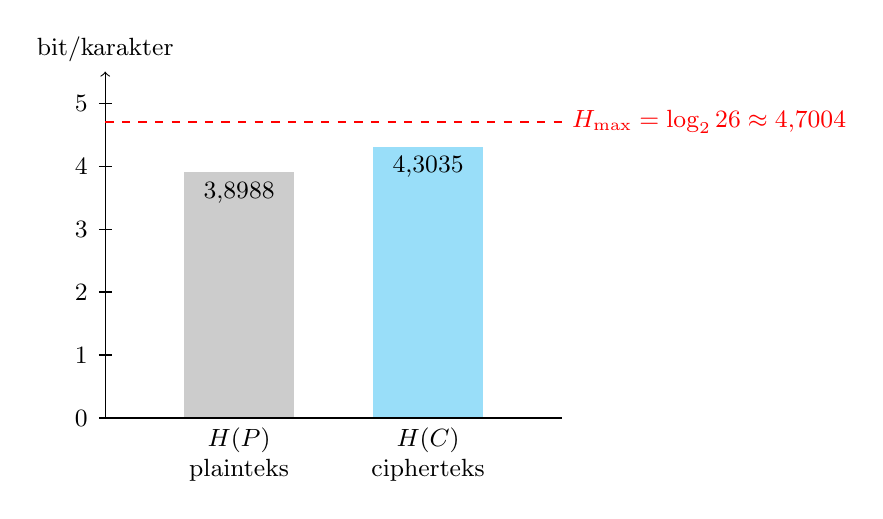
\begin{tikzpicture}[yscale=0.8, font=\small]
  \fill[gray!40] (1.0,0) rectangle (2.4,3.8988);
  \fill[cyan!40] (3.4,0) rectangle (4.8,4.3035);
  \node[below] at (1.7,3.8988) {3,8988};
  \node[below] at (4.1,4.3035) {4,3035};
  \draw[->] (0,0) -- (0,5.5) node[above] {bit/karakter};
  \draw (0,0) -- (5.8,0);
  \foreach \y in {0,...,5} {
    \draw (-0.08,\y) -- (0.08,\y);
    \node[left] at (-0.1,\y) {\y};
  }
  \draw[dashed, red, thick] (0,4.7004) -- (5.8,4.7004) node[right] {$H_{\max} = \log_2 26 \approx 4{,}7004$};
  \node[below, align=center] at (1.7,0) {$H(P)$\\plainteks};
  \node[below, align=center] at (4.1,0) {$H(C)$\\cipherteks};
\end{tikzpicture}\\[2pt]
{\small (c) Entropi plainteks dan cipherteks dibandingkan dengan entropi maksimum}
\caption{Enkripsi menaikkan entropi: cipherteks mencapai sekitar 91,55\% dari entropi maksimum teks 26 huruf \cite{munir_slides_itb}.}
\label{fig:entropi-ternate}
\end{figure}

\begin{contoh}
\begin{itemize}
  \item Entropi plaintext: $H(P) = 3{,}8988$ bit/karakter.
  \item Entropi ciphertext: $H(C) = 4{,}3035$ bit/karakter.
  \item Ciphertext mencapai $\dfrac{4{,}3035}{4{,}7004} \times 100\% \approx 91{,}55\%$ dari entropi maksimum teks 26 huruf.
\end{itemize}
Enkripsi menaikkan entropi: distribusi huruf pada ciphertext menjadi jauh lebih merata dibanding plaintext.
\end{contoh}

\subsection{Laju Bahasa dan Redundansi}

\textbf{Laju bahasa} (\textit{language rate}) adalah entropi per simbol dalam teks nyata suatu bahasa. Bahasa Inggris memiliki laju sekitar 1{,}0--1{,}5 bit/huruf, jauh di bawah $H_{\max} \approx 4{,}7$ bit/huruf \cite{shannon1951}.

\textbf{Redundansi} didefinisikan sebagai:
\[
R = 1 - \frac{H_{\text{aktual}}}{H_{\text{maksimum}}}
\]
Untuk perkiraan $H_{\text{aktual}} \approx 1{,}5$ dan $H_{\max} \approx 4{,}7$: $R \approx 0{,}68$ (sekitar 68\%). Redundansi inilah yang memungkinkan \textit{analisis frekuensi} memecah cipher substitusi monoalfabetik.

\begin{table}[htbp]
\centering
\small
\begin{tabular}{lcc}
\toprule
Sumber & Entropi Maksimum & Entropi Aktual \\
\midrule
Alfabet seragam (26 huruf) & 4{,}7 bit & 4{,}7 bit \\
Bahasa Inggris & 4{,}7 bit & $\approx$1{,}5 bit \\
Biner seragam & 1{,}0 bit & 1{,}0 bit \\
\bottomrule
\end{tabular}
\caption{Perbandingan entropi maksimum vs aktual.}
\end{table}

\begin{figure}[htbp]
\centering
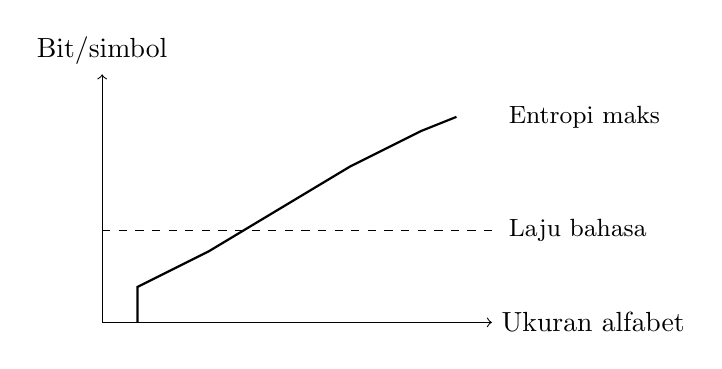
\begin{tikzpicture}[scale=0.9]
  \draw[->] (0,0) -- (5.5,0) node[right] {Ukuran alfabet};
  \draw[->] (0,0) -- (0,3.5) node[above] {Bit/simbol};
  \draw[thick] (0.5,0) -- (0.5,0.5) -- (1.5,1) -- (2.5,1.6) -- (3.5,2.2) -- (4.5,2.7) -- (5,2.9);
  \draw[dashed] (0,1.3) -- (5.5,1.3);
  \node[right, font=\small] at (5.6,2.9) {Entropi maks};
  \node[right, font=\small] at (5.6,1.3) {Laju bahasa};
\end{tikzpicture}
\caption{Ilustrasi: entropi maksimum naik dengan ukuran alfabet; laju bahasa aktual lebih rendah karena redundansi.}
\end{figure}

Cipher yang ideal menghasilkan ciphertext dengan entropi tinggi dan redundansi rendah sehingga penyerang sulit memanfaatkan pola bahasa.

\subsection{Pengayaan: Unicity Distance dan Perfect Secrecy}

\begin{catatan}
Subbagian ini bersifat \textbf{pengayaan} dan bukan prasyarat Sub-CPMK 2.3. Manfaatnya terasa saat membahas kriptanalisis cipher klasik (Bab~IV) dan desain cipher modern (Bab~V).
\end{catatan}

\textbf{Unicity distance} adalah panjang ciphertext minimum di mana hanya ada satu plaintext yang masuk akal yang dapat menghasilkan ciphertext tersebut \cite{shannon1949}. Untuk cipher dengan entropi kunci $H(K)$ dan redundansi per simbol $D$:
\[
U = \frac{H(K)}{D}
\]

\begin{contoh}
Untuk Caesar cipher:
\begin{itemize}
  \item Ruang kunci: 25 kemungkinan; $H(K) = \log_2 25 \approx 4{,}64$ bit
  \item Redundansi bahasa Inggris: $D \approx 4{,}7 - 1{,}5 = 3{,}2$ bit/huruf
  \item $U \approx 4{,}64 / 3{,}2 \approx 1{,}45$ huruf --- secara teoretis hanya perlu sedikit ciphertext untuk memecahkan Caesar secara unik
\end{itemize}
\end{contoh}

\begin{table}[htbp]
\centering
\small
\begin{tabular}{lcc}
\toprule
Cipher & Ukuran Kunci & Unicity Distance \\
\midrule
Caesar (25 kunci) & 4{,}64 bit & $\approx$2 huruf \\
Vigen\`{e}re ($26^k$ kunci) & $k \cdot 4{,}7$ bit & $\approx 1{,}5k$ huruf \\
DES (56-bit) & 56 bit & $\approx$17{,}5 huruf \\
AES-128 & 128 bit & $\approx$40 huruf \\
\bottomrule
\end{tabular}
\caption{Unicity distance untuk berbagai cipher (perkiraan).}
\end{table}

\begin{catatan}
Unicity distance adalah batas teoretis tentang berapa banyak ciphertext yang secara informasi cukup untuk menentukan kunci, bukan ukuran kemudahan serangan. Memecahkan AES tetap tidak layak secara komputasi walaupun unicity distance-nya hanya sekitar 40 huruf.
\end{catatan}

\textbf{Perfect secrecy} terjadi ketika ciphertext tidak memberikan informasi apa pun tentang plaintext. Shannon membuktikan syarat perlunya $H(K) \geq H(P)$. One-Time Pad memenuhinya jika kunci acak sepanjang plaintext dan hanya dipakai sekali. Definisi formal \textit{perfect secrecy}, pembuktiannya untuk OTP, serta alasan OTP tidak praktis dibahas pada subbab One-Time Pad di Bab~IV.

\begin{contoh}
Plaintext 8-bit dan kunci acak 8-bit di-XOR menghasilkan ciphertext; setiap kunci yang mungkin memberi ciphertext berbeda sehingga ciphertext saja tidak mengungkap plaintext.
\end{contoh}

Implikasi untuk desain cipher:
\begin{enumerate}
  \item \textbf{Kerentanan analisis frekuensi}: redundansi bahasa alami membuat cipher substitusi rentan.
  \item \textbf{Kebutuhan ruang kunci yang besar}: kunci pendek mudah dicari secara menyeluruh (\textit{brute force}).
  \item \textbf{Confusion dan diffusion} (Shannon): \textit{confusion} menyembunyikan hubungan antara kunci dan ciphertext; \textit{diffusion} menyebar pengaruh satu bit plaintext ke banyak bit ciphertext.
\end{enumerate}

\subsection{Koneksi ke Bab-Bab Berikutnya}

\begin{itemize}
  \item \textbf{Bab IV}: analisis frekuensi pada cipher klasik memanfaatkan redundansi bahasa
  \item \textbf{Bab V}: desain cipher modern menekankan confusion dan diffusion
  \item \textbf{Bab VI}: pemilihan ukuran kunci berkaitan dengan ruang kunci
\end{itemize}
